\documentclass[11pt]{standalone}
\usepackage{amssymb}
\usepackage{amsmath}
\usepackage[no-math]{fontspec}
\usepackage{unicode-math}
\setmainfont{Libertinus Sans}
\setsansfont{Libertinus Sans}
\setmathfont{Libertinus Math}
\usepackage{pgf,xcolor}
\usepackage{tikz}
\usetikzlibrary{arrows.meta, backgrounds}
\usepackage{pgfplots}
\pgfplotsset{compat=newest}
\usepackage{pifont}

\definecolor{my_darkgray}{HTML}{484949}
\definecolor{my_lightgray}{HTML}{F3F4F4}
\definecolor{my_darkblue}{HTML}{005A94}
\definecolor{my_lightblue}{HTML}{CCDEE9}
\definecolor{my_yellow}{HTML}{FFEC7F}
\definecolor{my_red}{HTML}{E60000}
\definecolor{my_orange}{HTML}{E87846}

\begin{document}
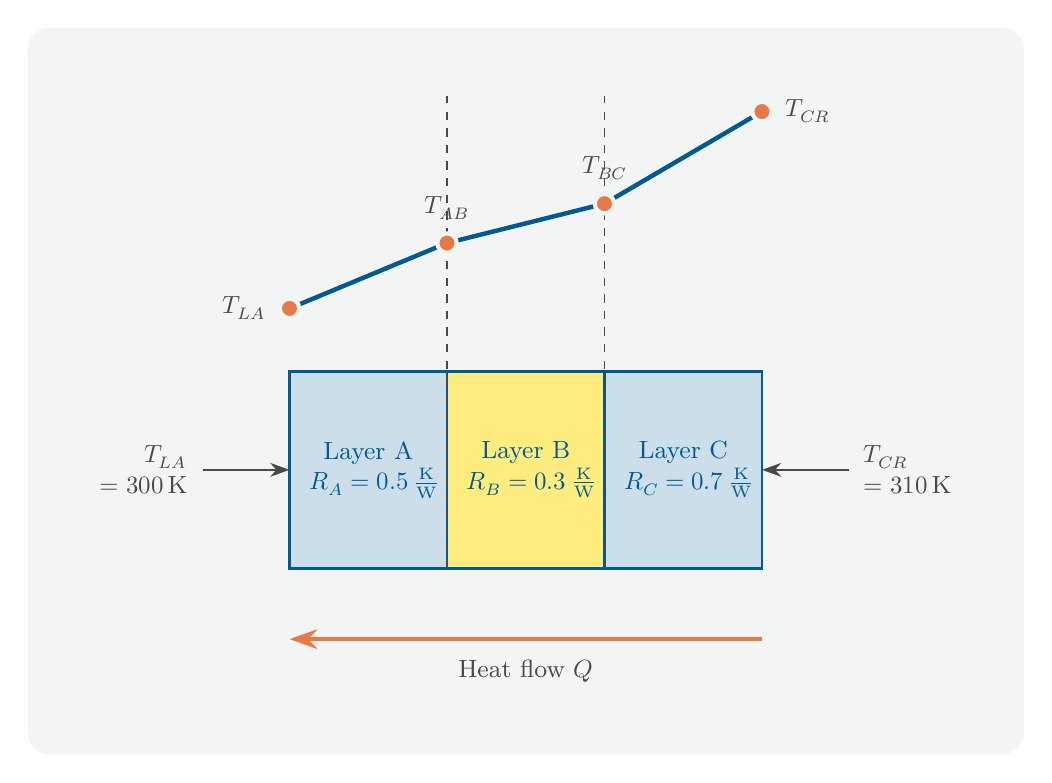
\begin{tikzpicture}[
    show background rectangle,
    background rectangle/.style={fill=my_lightgray, rounded corners=8pt},
    inner frame sep=0.8cm,
    annotation/.style={draw=my_darkgray, thick, -{Stealth[length=7pt, width=5pt]}}
]

% ==========================================================
% Koordinaten (x-Achse: schematische geometrische Position)
% Alle drei Schichten erhalten dieselbe Zeichenbreite (2 cm),
% da die tatsächlichen Dicken nicht gegeben sind.
% Bei gleicher Dicke ist die Steigung dT/dx proportional zu R_i:
%   Schicht A: R_A = 0,5 K/W  ->  mittlere Steigung
%   Schicht B: R_B = 0,3 K/W  ->  flachste Steigung
%   Schicht C: R_C = 0,7 K/W  ->  steilste Steigung
%
% Temperaturprofil (y, oberhalb der Wand):
%   Maßstab: 0,25 cm pro K, Nullpunkt bei T = 300 K
%   Profil-Basislinie: y = 3,3 cm (Wandhöhe 2,5 + Abstand 0,8)
%   T_LA = 300,00 K  ->  y = 3,30 cm
%   T_AB = 303,33 K  ->  y = 4,13 cm  (= 300 + 10 * 0,5/1,5)
%   T_BC = 305,33 K  ->  y = 4,63 cm  (= 300 + 10 * 0,8/1,5)
%   T_CR = 310,00 K  ->  y = 5,80 cm
% ==========================================================

% ----------------------------------------------------------
% Wandquerschnitt: drei Schichten, gleiche Zeichenbreite
% ----------------------------------------------------------

% Schicht A  (R_A = 0,5 K/W  ->  Breite 2,0 cm, schematisch)
\fill[fill=my_lightblue, draw=my_darkblue, line width=1pt]
    (0,0) rectangle (2.0,2.5);
\node[font=\small, text=my_darkblue, align=center] at (1.0,1.25)
    {Layer~A \\ \enspace $R_A = 0.5\,\tfrac{\mathrm{K}}{\mathrm{W}}$};

% Schicht B  (R_B = 0,3 K/W  ->  Breite 2,0 cm, schematisch)
\fill[fill=my_yellow, draw=my_darkblue, line width=1pt]
    (2.0,0) rectangle (4.0,2.5);
\node[font=\small, text=my_darkblue, align=center] at (3.0,1.25)
    {Layer~B \\ \enspace $R_B = 0.3\,\tfrac{\mathrm{K}}{\mathrm{W}}$};

% Schicht C  (R_C = 0,7 K/W  ->  Breite 2,0 cm, schematisch)
\fill[fill=my_lightblue, draw=my_darkblue, line width=1pt]
    (4.0,0) rectangle (6.0,2.5);
\node[font=\small, text=my_darkblue, align=center] at (5.0,1.25)
    {Layer~C \\ \enspace $R_C = 0.7\,\tfrac{\mathrm{K}}{\mathrm{W}}$};

% Randtemperaturen als Annotationen
\draw[annotation] (-1.1,1.25) -- (0,1.25);
\node[left=2pt, font=\small, text=my_darkgray, align=right] at (-1.1,1.25)
    {$T_{LA}$\\$=300\,\mathrm{K}$};

\draw[annotation] (7.1,1.25) -- (6.0,1.25);
\node[right=2pt, font=\small, text=my_darkgray, align=left] at (7.1,1.25)
    {$T_{CR}$\\$=310\,\mathrm{K}$};

% ----------------------------------------------------------
% Gestrichelte Grenzflächenlinien (verbinden Wand und Profil)
% ----------------------------------------------------------
\draw[my_darkgray, dashed, thin] (2.0,0) -- (2.0,6.0);
\draw[my_darkgray, dashed, thin] (4.0,0) -- (4.0,6.0);

% ----------------------------------------------------------
% Temperaturprofil: stückweise linear, unterschiedliche Steigungen
%   Schicht B flachste Steigung (R_B kleinster Widerstand)
%   Schicht C steilste Steigung (R_C größter Widerstand)
% ----------------------------------------------------------
\draw[my_darkblue, ultra thick, line cap=round, line join=round]
    (0,   3.30)   % T_LA = 300,00 K
 -- (2.0, 4.13)   % T_AB = 303,33 K  (DeltaT_A = 3,33 K)
 -- (4.0, 4.63)   % T_BC = 305,33 K  (DeltaT_B = 2,00 K)
 -- (6.0, 5.80);  % T_CR = 310,00 K  (DeltaT_C = 4,67 K)

% Punkte an den Grenzflächen (my_orange, weißer Rand)
\foreach \px/\py in {0/3.30, 2.0/4.13, 4.0/4.63, 6.0/5.80} {
    \fill[my_orange, draw=my_lightgray, line width=1.5pt]
        (\px,\py) circle (3.5pt);
}

% Temperaturbeschriftungen am Profil
\node[left=5pt,  font=\small, text=my_darkgray] at (0,   3.30) {$T_{LA}$};
\node[above=5pt, font=\small, text=my_darkgray] at (2.0, 4.13) {$T_{AB}$};
\node[above=5pt, font=\small, text=my_darkgray] at (4.0, 4.63) {$T_{BC}$};
\node[right=5pt, font=\small, text=my_darkgray] at (6.0, 5.80) {$T_{CR}$};

% ----------------------------------------------------------
% Wärmestrom-Pfeil (rechts nach links, da T_CR > T_LA)
% ----------------------------------------------------------
\draw[my_orange, ultra thick, -{Stealth[length=10pt, width=7pt]}]
    (6.0,-0.9) -- (0,-0.9);
\node[below=4pt, font=\small, text=my_darkgray] at (3.0,-0.9)
    {Heat flow $Q$};

\end{tikzpicture}
\end{document}
